% tex/resultados/res_02_analise_visual.tex
\section{Análise Visual dos Resultados}
\label{sec:res_analise_visual}

\textbf{Análise Gráfica:} \\
Para complementar a análise quantitativa apresentada nas tabelas, esta seção explora as visualizações gráficas geradas durante a avaliação. Estes gráficos oferecem uma compreensão mais intuitiva tanto da validade da nossa metodologia experimental quanto do comportamento interno do modelo de recomendação.

\subsection{Validação da Metodologia de Personas}
\textbf{Explicação:} \\
Uma etapa fundamental antes de analisar o impacto das personas é validar se elas foram construídas de forma metodologicamente correta. A Figura \ref{fig:tsne_personas_tcc2} serve a este propósito. Ela utiliza a técnica de redução de dimensionalidade \textbf{t-SNE} para projetar os vetores de features de 2503 dimensões de todos os 2000 perfis em um espaço 2D, permitindo a visualização de suas relações de similaridade.

\begin{figure}[hbt]
    \centering
    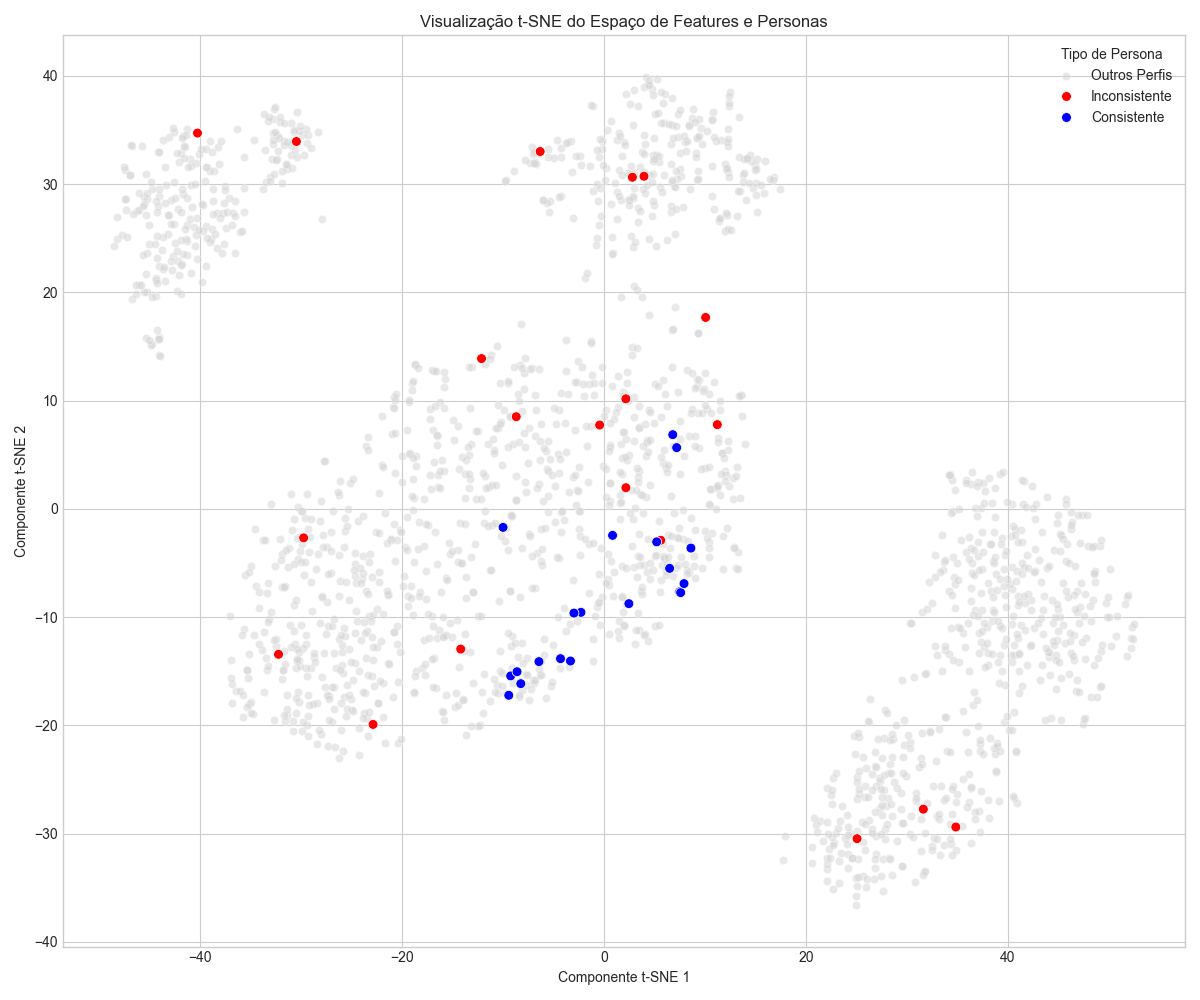
\includegraphics[width=0.9\textwidth]{imagens/embedding_space_personas.png} % IMPORTANTE: Verifique se o caminho "imagens/" está correto para o seu projeto
    \caption{Visualização t-SNE do espaço de features dos perfis. Os pontos azuis representam os perfis do histórico da Persona Consistente, e os vermelhos, da Persona Inconsistente.}
    \label{fig:tsne_personas_tcc2}
\end{figure}

\textbf{Interpretação da Figura \ref{fig:tsne_personas_tcc2}:} \\
A visualização confirma o sucesso da nossa abordagem de criação de personas. Os pontos em azul, que compõem o histórico da \textbf{Persona Consistente}, formam um agrupamento (cluster) coeso no espaço de embedding. Isso demonstra que os perfis selecionados para esta persona são, de fato, muito similares entre si, representando um usuário com um gosto bem definido. Em contraste, os pontos em vermelho, da \textbf{Persona Inconsistente}, aparecem totalmente dispersos pelo gráfico, sem formar nenhum padrão. Isso valida que eles foram selecionados de forma aleatória e representam um usuário com preferências diversas e não correlacionadas. Esta validação visual nos dá confiança para interpretar os resultados de desempenho a seguir.

\subsection{Análise da Distribuição de Probabilidades}
\textbf{Explicação:} \\
Para entender *como* o modelo chega às métricas de desempenho observadas, analisamos a distribuição de suas probabilidades de saída. A Figura \ref{fig:prob_dist_tcc2} exibe as curvas de densidade de probabilidade (KDE) para cada um dos três cenários experimentais. Em cada gráfico, a curva verde representa as probabilidades atribuídas a interações que foram um "Like" real, e a vermelha, a interações que foram um "Dislike" real.

\begin{figure}[hbt]
    \centering
    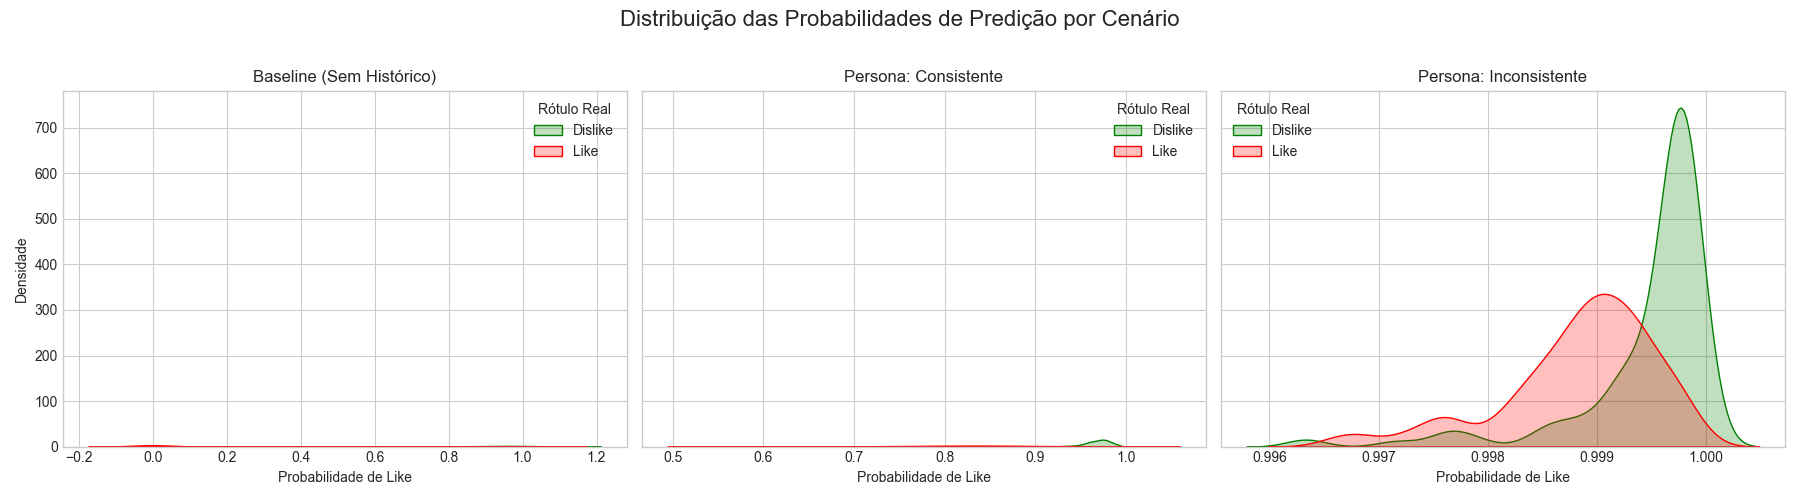
\includegraphics[width=\textwidth]{imagens/probability_distributions.png} % IMPORTANTE: Verifique se o caminho "imagens/" está correto
    \caption{Distribuição das probabilidades de predição para cada cenário, separadas por rótulo real (Verde: Like, Vermelho: Dislike).}
    \label{fig:prob_dist_tcc2}
\end{figure}

\textbf{Interpretação da Figura \ref{fig:prob_dist_tcc2}:}
\begin{itemize}
    \item \textbf{Cenário Baseline:} Observa-se uma separação quase perfeita entre as distribuições. A curva de "Likes" (verde) está concentrada em valores altos de probabilidade (próximos a 1.0), enquanto a curva de "Dislikes" (vermelha) está concentrada em valores muito baixos. Esta separação nítida é a representação visual de um AUC altíssimo (0.970) e de um modelo com alto poder de discriminação.
    
    \item \textbf{Cenário Persona Consistente:} Ocorre um fenômeno notável. Ambas as curvas, verde e vermelha, são deslocadas drasticamente para a direita. A curva de "Likes" se espreme ainda mais contra o valor 1.0. Crucialmente, a curva de "Dislikes" também se desloca, com uma grande parte de sua massa ultrapassando o limiar de 0.5. Isso ilustra visualmente por que o Recall se torna perfeito (todos os likes são classificados como > 0.5) e por que a Precisão cai (muitos dislikes também são classificados como > 0.5). O modelo, influenciado pelo histórico positivo, torna-se excessivamente otimista.

    \item \textbf{Cenário Persona Inconsistente:} O efeito é ainda mais extremo. Ambas as distribuições, verde e vermelha, colapsam quase inteiramente no valor 1.0. O modelo perde quase toda a sua capacidade de distinguir entre as duas classes com base em um limiar, atribuindo a probabilidade máxima a praticamente tudo. A pequena separação que ainda existe explica o AUC de 0.821 (ainda melhor que aleatório), mas para fins de classificação binária, o modelo se tornou inútil neste cenário.
\end{itemize}
Esta análise visual corrobora os dados das tabelas e fornece uma explicação intuitiva sobre como o contexto do usuário modula a confiança e o viés das predições do MatchPredict-AI.